\chapter{\textsuperscript{TC3} Cuadripolos}\label{chap:cuadripolos}
\section{Introducción}
\label{sec:org89dadb3}

\subsubsection{Cuadripolo}
\label{sec:org9ef7725}
\begin{center}
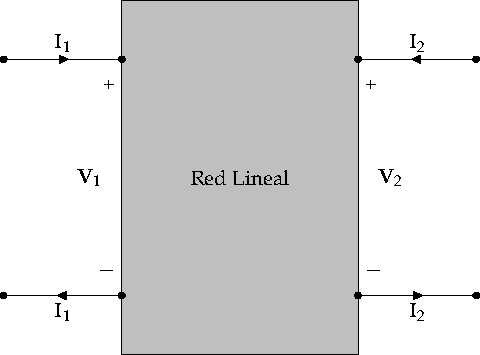
\includegraphics[height=5cm]{../figs/cuadripolo.pdf}
\end{center}

\begin{center}
\textbf{Atención al sentido de las corrientes}
\end{center}
\subsubsection{Cuadripolos Recíprocos y Simétricos}
\label{sec:org45c7b40}

\begin{itemize}
\item Un cuadripolo es \textbf{recíproco} si, al intercambiar la posición de las excitaciones, la respuesta en el puerto correspondiente no sufre cambios (teorema de reciprocidad).
\item Un cuadripolo lineal (RLC) y \textbf{sin fuentes dependientes} es recíproco.
\item Un \textbf{cuadripolo recíproco es simétrico} si se puede intercambiar la entrada con la salida (simetría física).
\end{itemize}
\section{Parámetros de Cuadripolos}
\label{sec:orgc7cab56}
\subsection{Parámetros de Impedancia}
\label{sec:org99c6d5d}

\subsubsection{Definición}
\label{sec:orga66e998}
\begin{center}
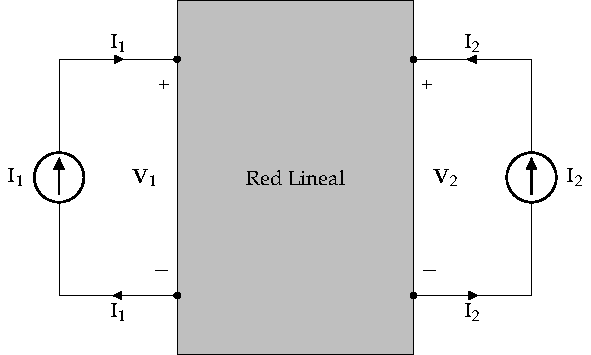
\includegraphics[height=4cm]{../figs/cuadripolo_fuentes_corriente.pdf}
\end{center}

Mediante teorema de superposición:
\[
\begin{array}{l}
  \mathbf{V}_1 = \mathbf{z}_{11} \mathbf{I}_1 + \mathbf{z}_{12} \mathbf{I}_2\\
  \mathbf{V}_2 = \mathbf{z}_{21} \mathbf{I}_1 + \mathbf{z}_{22} \mathbf{I}_2\\
\end{array}
\]

Las variables independientes (\emph{generadores}) son \(\mathbf{I}_1\) e \(\mathbf{I}_2\).

\subsubsection{Expresión Matricial}
\label{sec:orgf922a0b}
\begin{center}
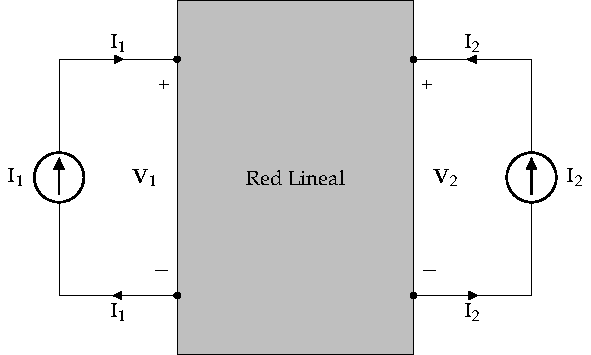
\includegraphics[height=4cm]{../figs/cuadripolo_fuentes_corriente.pdf}
\end{center}

\[
  \left[
    \begin{array}{c}
      \mathbf{V}_1\\
      \mathbf{V}_2
    \end{array}
  \right] =
  \left[
    \begin{array}{cc}
      \mathbf{z}_{11} & \mathbf{z}_{12}\\
      \mathbf{z}_{21} & \mathbf{z}_{22}
    \end{array}
  \right] \cdot
  \left[
    \begin{array}{c}
      \mathbf{I}_1\\
      \mathbf{I}_2
    \end{array}
  \right]
\]

\subsubsection{Circuito Equivalente}
\label{sec:org634cc26}
\begin{center}
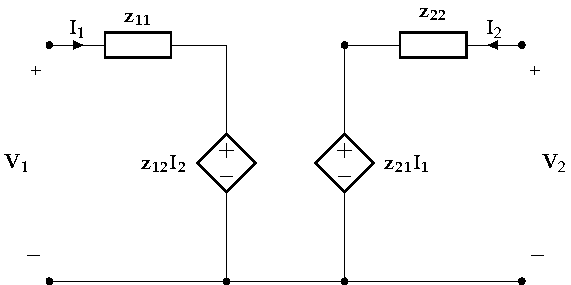
\includegraphics[height=4cm]{../figs/circuitoEquivalenteZ.pdf}
\end{center}

\[
\begin{array}{l}
  \mathbf{V}_1 = \mathbf{z}_{11} \mathbf{I}_1 + \mathbf{z}_{12} \mathbf{I}_2\\
  \mathbf{V}_2 = \mathbf{z}_{21} \mathbf{I}_1 + \mathbf{z}_{22} \mathbf{I}_2\\
\end{array}
\]

\subsubsection{Cálculo de parámetros}
\label{sec:org74b4bb2}

\begin{enumerate}
\item Salida en abierto
\label{sec:org2d081df}

\begin{enumerate}
\item \hfill{}\textsc{BMCOL}
\label{sec:orgb2e3e30}
\renewcommand{\arraystretch}{2}
\[
  \begin{array}{c}
    \mathbf{z}_{11} = \left.\frac{\mathbf{V}_1}{\mathbf{I}_1}\right\rvert_{\mathbf{I}_2 = 0} \\
    \mathbf{z}_{21} = \left.\frac{\mathbf{V}_2}{\mathbf{I}_1}\right\rvert_{\mathbf{I}_2 = 0}
  \end{array}
\]

\item \hfill{}\textsc{BMCOL}
\label{sec:orgd3d533a}
\begin{center}
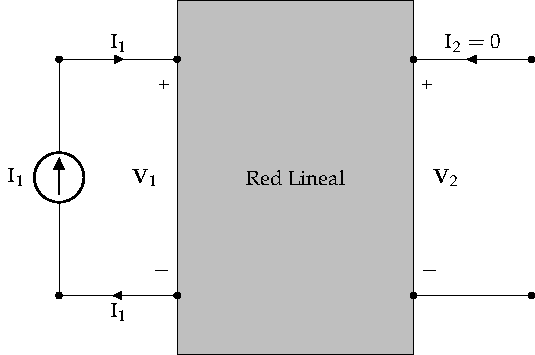
\includegraphics[height=4cm]{../figs/parametrosZ_entrada.pdf}
\end{center}
\end{enumerate}

\item \hfill{}\textsc{B\_ignoreheading}
\label{sec:orgb41b705}
\[
  \left[
    \begin{array}{c}
      \mathbf{V}_1\\
      \mathbf{V}_2
    \end{array}
  \right] =
  \left[
    \begin{array}{cc}
      \color{blue}{\mathbf{z}_{11}} & \mathbf{z}_{12}\\
      \color{blue}{\mathbf{z}_{21}} & \mathbf{z}_{22}
    \end{array}
  \right] \cdot
  \left[
    \begin{array}{c}
      \color{blue}{\mathbf{I}_1}\\
      \mathbf{I}_2
    \end{array}
  \right]
\]
\end{enumerate}

\subsubsection{Cálculo de parámetros}
\label{sec:org4ab5ebf}

\begin{enumerate}
\item Entrada en abierto
\label{sec:org16769ae}

\begin{enumerate}
\item \hfill{}\textsc{BMCOL}
\label{sec:org054439f}
\begin{center}
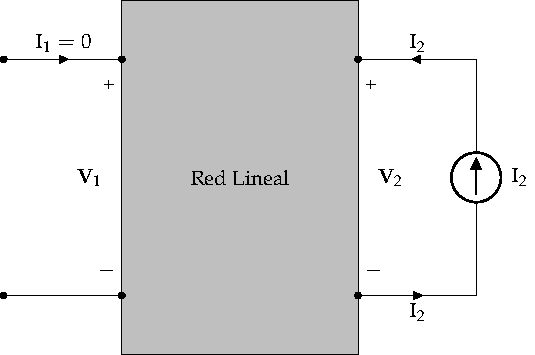
\includegraphics[height=4cm]{../figs/parametrosZ_salida.pdf}
\end{center}

\item \hfill{}\textsc{BMCOL}
\label{sec:orge6ceda7}
\renewcommand{\arraystretch}{2}
\[
  \begin{array}{c}
    \mathbf{z}_{12} = \left.\frac{\mathbf{V}_1}{\mathbf{I}_2}\right\rvert_{\mathbf{I}_1 = 0}\\
    \mathbf{z}_{22} = \left.\frac{\mathbf{V}_2}{\mathbf{I}_2}\right\rvert_{\mathbf{I}_1 = 0}
  \end{array}
\]
\end{enumerate}

\item \hfill{}\textsc{B\_ignoreheading}
\label{sec:org55c3206}
\[
  \left[
    \begin{array}{c}
      \mathbf{V}_1\\
      \mathbf{V}_2
    \end{array}
  \right] =
  \left[
    \begin{array}{cc}
      \mathbf{z}_{11} & \color{blue}{\mathbf{z}_{12}}\\
      \mathbf{z}_{21} & \color{blue}{\mathbf{z}_{22}}
    \end{array}
  \right] \cdot
  \left[
    \begin{array}{c}
      \mathbf{I}_1\\
      \color{blue}{\mathbf{I}_2}
    \end{array}
  \right]
\]
\end{enumerate}

\subsubsection{Reciprocidad}
\label{sec:org827c391}
\[
\left.\mathbf{V_1}\right\rvert_{
  \begin{array}{l}
\mathbf{I_1} = 0\\ \mathbf{I_2} = \mathbf{I_x}
  \end{array}
} =% 
\left.\mathbf{V_2}\right\rvert_{
  \begin{array}{l}
\mathbf{I_2} = 0\\ \mathbf{I_1} = \mathbf{I_x}
  \end{array}
}
\]

\begin{enumerate}
\item \hfill{}\textsc{BMCOL}
\label{sec:org664d831}
\begin{center}
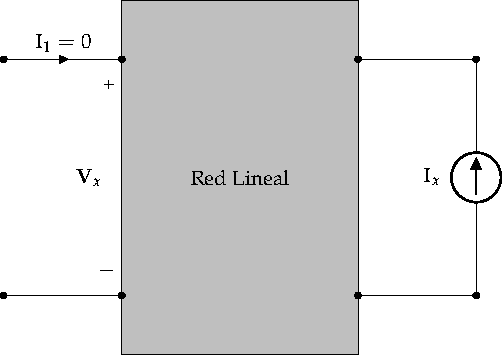
\includegraphics[height=4cm]{../figs/reciprocidadZ_entrada.pdf}
\end{center}
\item \hfill{}\textsc{BMCOL}
\label{sec:orge37f911}
\begin{center}
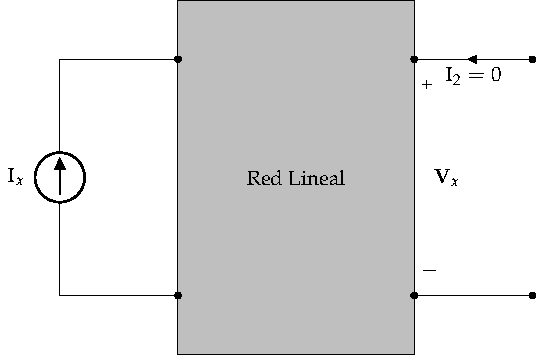
\includegraphics[height=4cm]{../figs/reciprocidadZ_salida.pdf}
\end{center}
\end{enumerate}
\subsubsection{Relación entre parámetros}
\label{sec:orgaf2fabb}
Las impedancias de transferencia son idénticas
\[
  \left.
    \begin{array}{l}
      \mathbf{V}_x = \mathbf{z}_{11} 0  + \mathbf{z}_{12} \mathbf{I}_x\\
      \mathbf{V}_x = \mathbf{z}_{21} \mathbf{I}_x + \mathbf{z}_{22} 0\\
    \end{array} \right\} \rightarrow \boxed{\mathbf{z_{12}} = \mathbf{z_{21}}}
\]

\begin{enumerate}
\item \hfill{}\textsc{BMCOL}
\label{sec:orgcc11e65}
\begin{center}
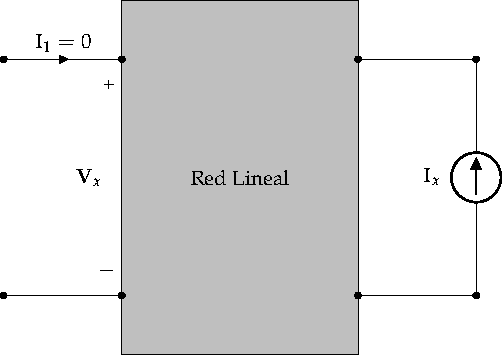
\includegraphics[height=4cm]{../figs/reciprocidadZ_entrada.pdf}
\end{center}
\item \hfill{}\textsc{BMCOL}
\label{sec:orgc53448d}
\begin{center}
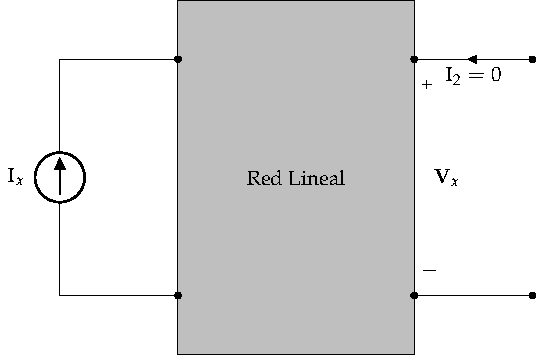
\includegraphics[height=4cm]{../figs/reciprocidadZ_salida.pdf}
\end{center}
\end{enumerate}

\subsubsection{Circuito Equivalente en T}
\label{sec:orgf4a859d}

\[
\boxed{\mathbf{z_{12}} = \mathbf{z_{21}}}
\rightarrow
\left[
    \begin{array}{c}
      \mathbf{V}_1\\
      \mathbf{V}_2
    \end{array}
  \right] =
  \left[
    \begin{array}{cc}
      \mathbf{z}_{11} & \color{red}{\mathbf{z}_{12}}\\
      \color{red}{\mathbf{z}_{12}} & \mathbf{z}_{22}
    \end{array}
  \right] \cdot
  \left[
    \begin{array}{c}
      \mathbf{I}_1\\
      \mathbf{I}_2
    \end{array}
  \right]
\]

\begin{enumerate}
\item Ejercicio
\label{sec:org3cfa18b}
Demostrar que un cuadripolo recíproco es equivalente al circuito en T de la figura.
\begin{center}
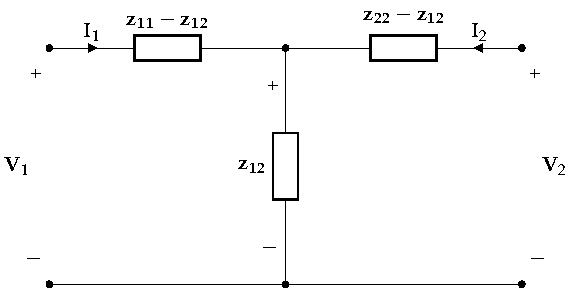
\includegraphics[height=4cm]{../figs/circuitoEquivalenteZReciproco.pdf}
\end{center}
\end{enumerate}

\subsubsection{Cuadripolo Simétrico}
\label{sec:orga8e8529}
\begin{center}
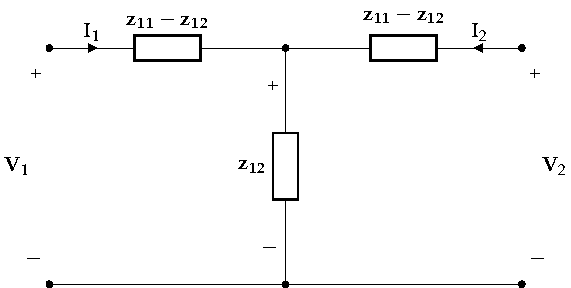
\includegraphics[height=4cm]{../figs/circuitoEquivalenteZSimetrico.pdf}
\end{center}

\[
\boxed{\mathbf{z_{11}} = \mathbf{z_{22}}}
\rightarrow
\left[
    \begin{array}{c}
      \mathbf{V}_1\\
      \mathbf{V}_2
    \end{array}
  \right] =
  \left[
    \begin{array}{cc}
      \color{blue}{\mathbf{z}_{11}} & \color{red}{\mathbf{z}_{12}}\\
      \color{red}{\mathbf{z}_{12}} & \color{blue}{\mathbf{z}_{11}}
    \end{array}
  \right] \cdot
  \left[
    \begin{array}{c}
      \mathbf{I}_1\\
      \mathbf{I}_2
    \end{array}
  \right]
\]


\subsubsection{No siempre hay parámetros Z}
\label{sec:orga3d8e88}

¿Cuáles son los parámetros Z \ldots{} 

\begin{itemize}
\item de un transformador ideal?
\item de una impedancia serie?
\end{itemize}

\subsection{Parámetros de Admitancia}
\label{sec:orgf2edf7b}
\subsubsection{Definición}
\label{sec:org4be9299}
\begin{center}
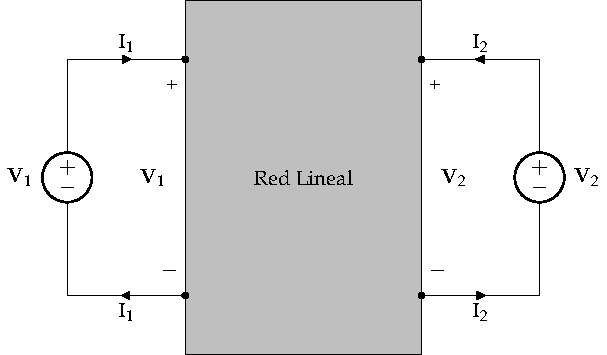
\includegraphics[height=4cm]{../figs/cuadripolo_fuentes_tension.pdf}
\end{center}

Mediante teorema de superposición:
\[
\begin{array}{l}
  \mathbf{I}_1 = \mathbf{y}_{11} \mathbf{V}_1 + \mathbf{y}_{12} \mathbf{V}_2\\
  \mathbf{I}_2 = \mathbf{y}_{21} \mathbf{V}_1 + \mathbf{y}_{22} \mathbf{V}_2\\
\end{array}
\]

Las variables independientes (\emph{generadores}) son \(\mathbf{V}_1\) e \(\mathbf{V}_2\).

\subsubsection{Expresión Matricial}
\label{sec:org3731aa9}
\begin{center}
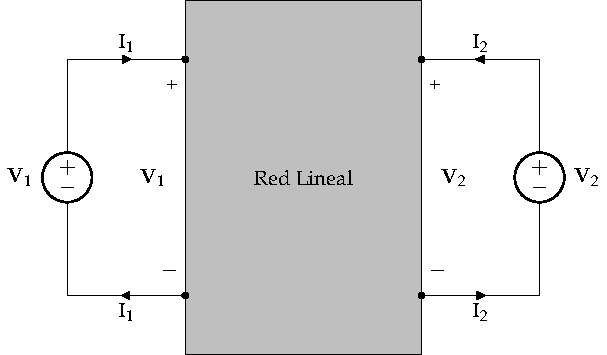
\includegraphics[height=4cm]{../figs/cuadripolo_fuentes_tension.pdf}
\end{center}

\[
  \left[
    \begin{array}{c}
      \mathbf{I}_1\\
      \mathbf{I}_2
    \end{array}
  \right] =
  \left[
    \begin{array}{cc}
      \mathbf{y}_{11} & \mathbf{y}_{12}\\
      \mathbf{y}_{21} & \mathbf{y}_{22}
    \end{array}
  \right] \cdot
  \left[
    \begin{array}{c}
      \mathbf{V}_1\\
      \mathbf{V}_2
    \end{array}
  \right]
\]

\subsubsection{Circuito Equivalente}
\label{sec:orgc722f4f}
\begin{center}
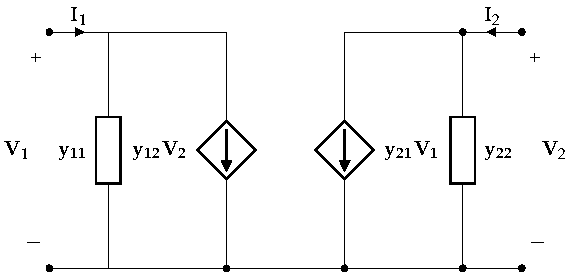
\includegraphics[height=4cm]{../figs/circuitoEquivalenteY.pdf}
\end{center}

\[
\begin{array}{l}
  \mathbf{I}_1 = \mathbf{y}_{11} \mathbf{V}_1 + \mathbf{y}_{12} \mathbf{V}_2\\
  \mathbf{I}_2 = \mathbf{y}_{21} \mathbf{V}_1 + \mathbf{y}_{22} \mathbf{V}_2\\
\end{array}
\]


\subsubsection{Cálculo de parámetros}
\label{sec:org003b72b}

\begin{enumerate}
\item Salida en cortocircuito
\label{sec:orgb1789af}

\begin{enumerate}
\item \hfill{}\textsc{BMCOL}
\label{sec:org0edf562}
\renewcommand{\arraystretch}{2}
\[
  \begin{array}{c}
    \mathbf{y}_{11} = \left.\frac{\mathbf{I}_1}{\mathbf{V}_1}\right\rvert_{\mathbf{V}_2 = 0} \\
    \mathbf{y}_{21} = \left.\frac{\mathbf{I}_2}{\mathbf{V}_1}\right\rvert_{\mathbf{V}_2 = 0}
  \end{array}
\]

\item \hfill{}\textsc{BMCOL}
\label{sec:org7c2d782}
\begin{center}
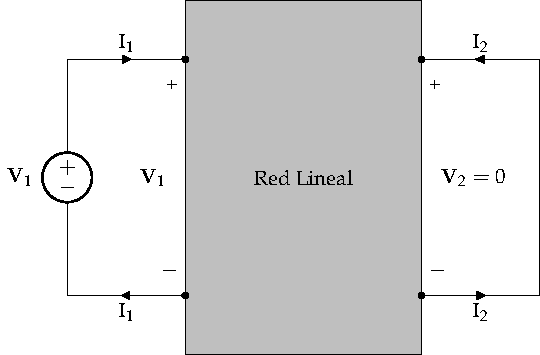
\includegraphics[height=4cm]{../figs/parametrosY_entrada.pdf}
\end{center}
\end{enumerate}

\item \hfill{}\textsc{B\_ignoreheading}
\label{sec:orgce1c711}
\[
  \left[
    \begin{array}{c}
      \mathbf{I}_1\\
      \mathbf{I}_2
    \end{array}
  \right] =
  \left[
    \begin{array}{cc}
      \color{blue}{\mathbf{y}_{11}} & \mathbf{y}_{12}\\
      \color{blue}{\mathbf{y}_{21}} & \mathbf{y}_{22}
    \end{array}
  \right] \cdot
  \left[
    \begin{array}{c}
      \color{blue}{\mathbf{V}_1}\\
      \mathbf{V}_2
    \end{array}
  \right]
\]
\end{enumerate}


\subsubsection{Cálculo de parámetros}
\label{sec:org7676724}

\begin{enumerate}
\item Entrada en cortocircuito
\label{sec:org1d8c65d}

\begin{enumerate}
\item \hfill{}\textsc{BMCOL}
\label{sec:orgda9e197}
\begin{center}
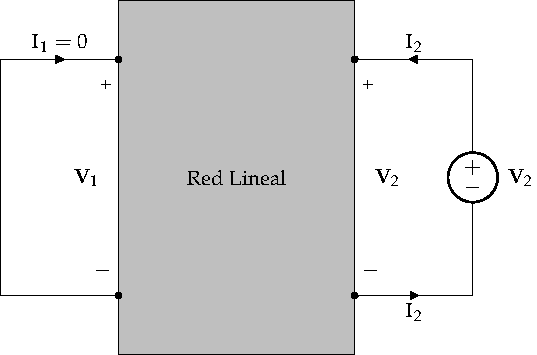
\includegraphics[height=4cm]{../figs/parametrosY_salida.pdf}
\end{center}

\item \hfill{}\textsc{BMCOL}
\label{sec:org35720cd}
\renewcommand{\arraystretch}{2}
\[
  \begin{array}{c}
    \mathbf{y}_{12} = \left.\frac{\mathbf{I}_1}{\mathbf{V}_2}\right\rvert_{\mathbf{V}_1 = 0}\\
    \mathbf{y}_{22} = \left.\frac{\mathbf{I}_2}{\mathbf{V}_2}\right\rvert_{\mathbf{V}_1 = 0}
  \end{array}
\]
\end{enumerate}

\item \hfill{}\textsc{B\_ignoreheading}
\label{sec:org5814116}
\[
  \left[
    \begin{array}{c}
      \mathbf{I}_1\\
      \mathbf{I}_2
    \end{array}
  \right] =
  \left[
    \begin{array}{cc}
      \mathbf{y}_{11} & \color{blue}{\mathbf{y}_{12}}\\
      \mathbf{y}_{21} & \color{blue}{\mathbf{y}_{22}}
    \end{array}
  \right] \cdot
  \left[
    \begin{array}{c}
      \mathbf{V}_1\\
      \color{blue}{\mathbf{V}_2}
    \end{array}
  \right]
\]
\end{enumerate}

\subsubsection{Reciprocidad}
\label{sec:orge3f94a7}

\[
\mathbf{I_1}\rvert_{
  \begin{array}{l}
\mathbf{V_1} = 0 \\ \mathbf{V_2} = \mathbf{V_x}
  \end{array}
} =% 
\mathbf{I_2}\rvert_{
  \begin{array}{l}
\mathbf{V_2} = 0 \\ \mathbf{V_1} = \mathbf{V_x}
  \end{array}
}
\]

\begin{enumerate}
\item \hfill{}\textsc{BMCOL}
\label{sec:orgbafb0fe}
\begin{center}
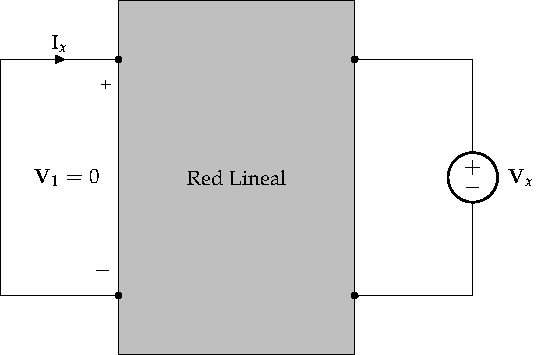
\includegraphics[height=4cm]{../figs/reciprocidadY_entrada.pdf}
\end{center}
\item \hfill{}\textsc{BMCOL}
\label{sec:orgb4d144b}
\begin{center}
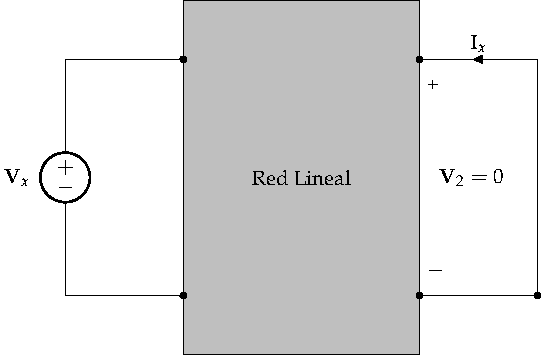
\includegraphics[height=4cm]{../figs/reciprocidadY_salida.pdf}
\end{center}
\end{enumerate}
\subsubsection{Relación entre parámetros}
\label{sec:org5379fea}
Las admitancias de transferencia son idénticas
\[
  \left.
    \begin{array}{l}
      \mathbf{I}_x = \mathbf{y}_{11} 0  + \mathbf{y}_{12} \mathbf{V}_x\\
      \mathbf{I}_x = \mathbf{y}_{21} \mathbf{V}_x + \mathbf{y}_{22} 0\\
    \end{array} \right\} \rightarrow \boxed{\mathbf{y_{12}} = \mathbf{y_{21}}}
\]

\begin{enumerate}
\item \hfill{}\textsc{BMCOL}
\label{sec:org6237778}
\begin{center}
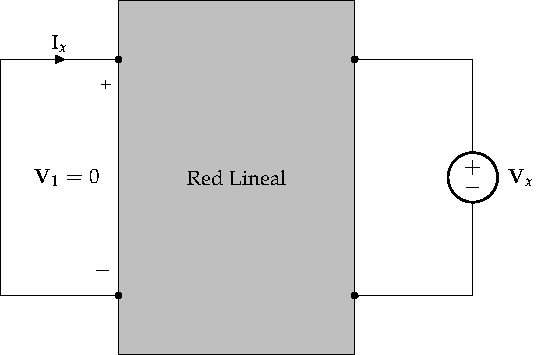
\includegraphics[height=4cm]{../figs/reciprocidadY_entrada.pdf}
\end{center}
\item \hfill{}\textsc{BMCOL}
\label{sec:orgf1cf80d}
\begin{center}
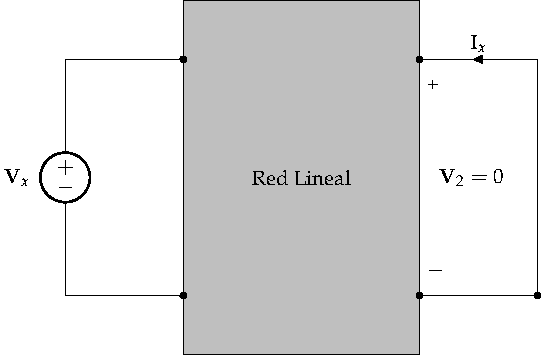
\includegraphics[height=4cm]{../figs/reciprocidadY_salida.pdf}
\end{center}
\end{enumerate}
\subsubsection{Circuito Equivalente en \(\pi\)}
\label{sec:org2f3cf9b}
\[
\boxed{\mathbf{y_{12}} = \mathbf{y_{21}}}
\rightarrow
\left[
    \begin{array}{c}
      \mathbf{I}_1\\
      \mathbf{I}_2
    \end{array}
  \right] =
  \left[
    \begin{array}{cc}
      \mathbf{y}_{11} & \color{red}{\mathbf{y}_{12}}\\
      \color{red}{\mathbf{y}_{12}} & \mathbf{y}_{22}
    \end{array}
  \right] \cdot
  \left[
    \begin{array}{c}
      \mathbf{V}_1\\
      \mathbf{V}_2
    \end{array}
  \right]
\]

\begin{enumerate}
\item Ejercicio
\label{sec:orgeb5b5d1}
Demostrar que un cuadripolo recíproco es equivalente al circuito en \(\pi\) de la figura.
\begin{center}
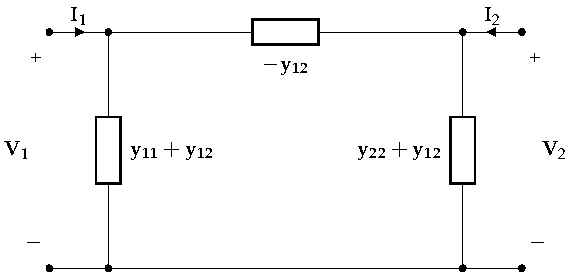
\includegraphics[height=4cm]{../figs/circuitoEquivalenteYReciproco.pdf}
\end{center}
\end{enumerate}

\subsubsection{Cuadripolo Simétrico}
\label{sec:orgbe5cf36}

\begin{center}
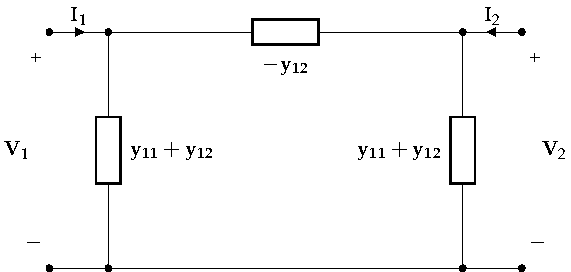
\includegraphics[height=4cm]{../figs/circuitoEquivalenteYSimetrico.pdf}
\end{center}


\[
\boxed{\mathbf{y_{11}} = \mathbf{y_{22}}}
\rightarrow
\left[
    \begin{array}{c}
      \mathbf{I}_1\\
      \mathbf{I}_2
    \end{array}
  \right] =
  \left[
    \begin{array}{cc}
      \color{blue}{\mathbf{y}_{11}} & \color{red}{\mathbf{y}_{12}}\\
      \color{red}{\mathbf{y}_{12}} & \color{blue}{\mathbf{y}_{11}}
    \end{array}
  \right] \cdot
  \left[
    \begin{array}{c}
      \mathbf{V}_1\\
      \mathbf{V}_2
    \end{array}
  \right]
\]


\subsubsection{No siempre hay parámetros Y}
\label{sec:org4af051f}

¿Cuáles son los parámetros Y \ldots{} 

\begin{itemize}
\item de un transformador ideal?
\item de una impedancia paralelo?
\end{itemize}

\subsection{Parámetros Híbridos}
\label{sec:org7054e38}
\subsubsection{Definición}
\label{sec:orgafed8ae}
\begin{center}
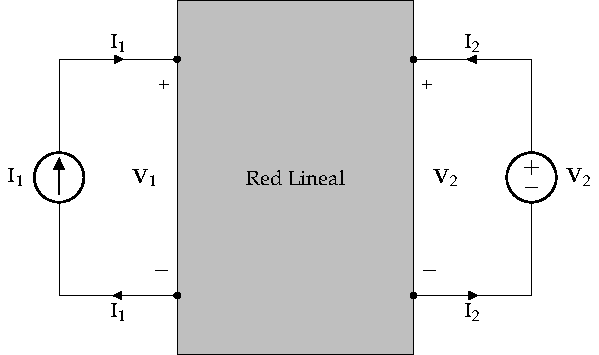
\includegraphics[height=4cm]{../figs/cuadripolo_hibrido.pdf}
\end{center}

Mediante teorema de superposición:
\[
\begin{array}{l}
  \mathbf{V}_1 = \mathbf{h}_{11} \mathbf{I}_1 + \mathbf{h}_{12} \mathbf{V}_2\\
  \mathbf{I}_2 = \mathbf{h}_{21} \mathbf{I}_1 + \mathbf{h}_{22} \mathbf{V}_2\\
\end{array}
\]

Las variables independientes (\emph{generadores}) son \(\mathbf{I}_1\) e \(\mathbf{V}_2\).


\subsubsection{Expresión Matricial}
\label{sec:org249baea}
\begin{center}
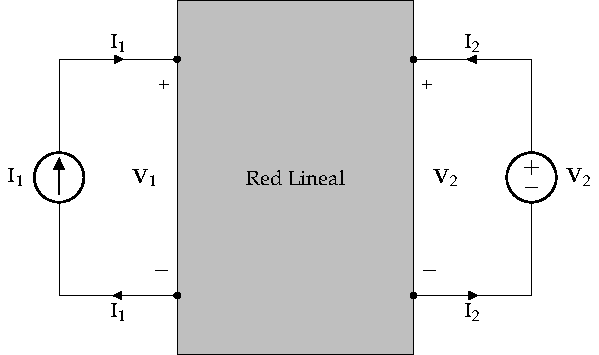
\includegraphics[height=4cm]{../figs/cuadripolo_hibrido.pdf}
\end{center}

\[
  \left[
    \begin{array}{c}
      \mathbf{V}_1\\
      \mathbf{I}_2
    \end{array}
  \right] =
  \left[
    \begin{array}{cc}
      \mathbf{h}_{11} & \mathbf{h}_{12}\\
      \mathbf{h}_{21} & \mathbf{h}_{22}
    \end{array}
  \right] \cdot
  \left[
    \begin{array}{c}
      \mathbf{I}_1\\
      \mathbf{V}_2
    \end{array}
  \right]
\]

\subsubsection{Circuito Equivalente}
\label{sec:org18f3f5d}
\begin{center}
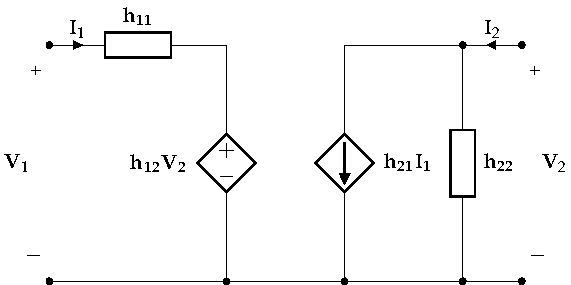
\includegraphics[height=4cm]{../figs/circuitoEquivalenteH.pdf}
\end{center}

\[
\begin{array}{l}
  \mathbf{V}_1 = \mathbf{h}_{11} \mathbf{I}_1 + \mathbf{h}_{12} \mathbf{V}_2\\
  \mathbf{I}_2 = \mathbf{h}_{21} \mathbf{I}_1 + \mathbf{h}_{22} \mathbf{V}_2\\
\end{array}
\]

\subsubsection{Cálculo de parámetros}
\label{sec:org2210706}

\begin{enumerate}
\item Salida en cortocircuito
\label{sec:org8fc619b}

\begin{enumerate}
\item \hfill{}\textsc{BMCOL}
\label{sec:orgebc69c6}
\renewcommand{\arraystretch}{2}
\[
  \begin{array}{c}
    \mathbf{h}_{11} = \left.\frac{\mathbf{V}_1}{\mathbf{I}_1}\right\rvert_{\mathbf{V}_2 = 0} \\
    \mathbf{h}_{21} = \left.\frac{\mathbf{I}_2}{\mathbf{I}_1}\right\rvert_{\mathbf{V}_2 = 0}
  \end{array}
\]

\item \hfill{}\textsc{BMCOL}
\label{sec:org3dc9d0b}
\begin{center}
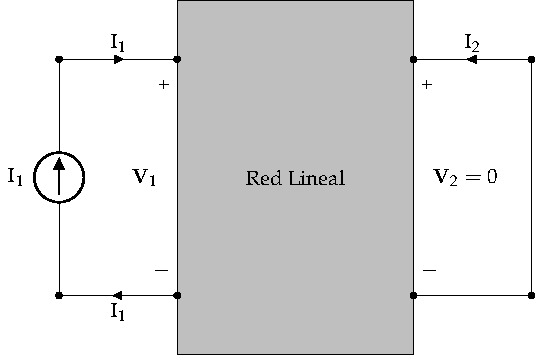
\includegraphics[height=4cm]{../figs/parametrosH_entrada.pdf}
\end{center}
\end{enumerate}

\item \hfill{}\textsc{B\_ignoreheading}
\label{sec:org2feac24}
\[
  \left[
    \begin{array}{c}
      \mathbf{V}_1\\
      \mathbf{I}_2
    \end{array}
  \right] =
  \left[
    \begin{array}{cc}
      \color{blue}{\mathbf{h}_{11}} & \mathbf{h}_{12}\\
      \color{blue}{\mathbf{h}_{21}} & \mathbf{h}_{22}
    \end{array}
  \right] \cdot
  \left[
    \begin{array}{c}
      \color{blue}{\mathbf{I}_1}\\
      \mathbf{V}_2
    \end{array}
  \right]
\]
\end{enumerate}

\subsubsection{Cálculo de parámetros}
\label{sec:org16f02aa}

\begin{enumerate}
\item Entrada en abierto
\label{sec:orgc4ee659}

\begin{enumerate}
\item \hfill{}\textsc{BMCOL}
\label{sec:org4eea1be}
\begin{center}
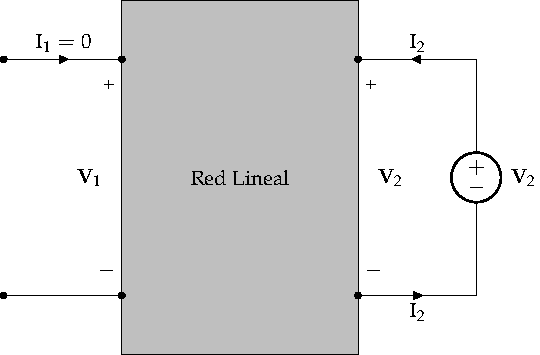
\includegraphics[height=4cm]{../figs/parametrosH_salida.pdf}
\end{center}

\item \hfill{}\textsc{BMCOL}
\label{sec:org3452f57}
\renewcommand{\arraystretch}{2}
\[
  \begin{array}{c}
    \mathbf{h}_{12} = \left.\frac{\mathbf{V}_1}{\mathbf{V}_2}\right\rvert_{\mathbf{I}_1 = 0}\\
    \mathbf{h}_{22} = \left.\frac{\mathbf{I}_2}{\mathbf{V}_2}\right\rvert_{\mathbf{I}_1 = 0}
  \end{array}
\]
\end{enumerate}

\item \hfill{}\textsc{B\_ignoreheading}
\label{sec:org9431e69}
\[
  \left[
    \begin{array}{c}
      \mathbf{V}_1\\
      \mathbf{I}_2
    \end{array}
  \right] =
  \left[
    \begin{array}{cc}
      \mathbf{h}_{11} & \color{blue}{\mathbf{h}_{12}}\\
      \mathbf{h}_{21} & \color{blue}{\mathbf{h}_{22}}
    \end{array}
  \right] \cdot
  \left[
    \begin{array}{c}
      \mathbf{I}_1\\
      \color{blue}{\mathbf{V}_2}
    \end{array}
  \right]
\]
\end{enumerate}


\subsection{Parámetros Híbridos Inversos}
\label{sec:orgbbd88b6}

\subsubsection{Definición}
\label{sec:org40235ae}
\begin{center}
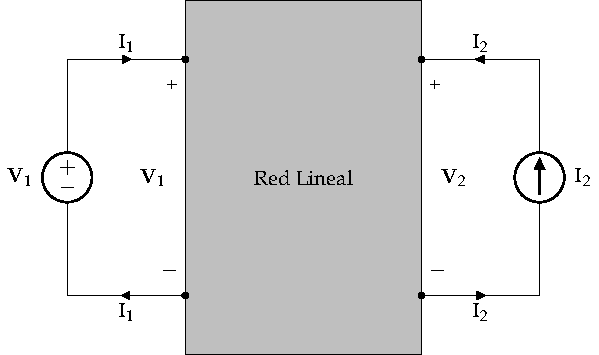
\includegraphics[height=4cm]{../figs/cuadripolo_hibrido_inverso.pdf}
\end{center}

Mediante teorema de superposición:
\[
\begin{array}{l}
  \mathbf{I}_1 = \mathbf{g}_{11} \mathbf{V}_1 + \mathbf{g}_{12} \mathbf{I}_2\\
  \mathbf{V}_2 = \mathbf{g}_{21} \mathbf{V}_1 + \mathbf{g}_{22} \mathbf{I}_2\\
\end{array}
\]

Las variables independientes (\emph{generadores}) son \(\mathbf{V}_1\) e \(\mathbf{I}_2\).

\subsubsection{Expresión Matricial}
\label{sec:org5bc2ad0}
\begin{center}
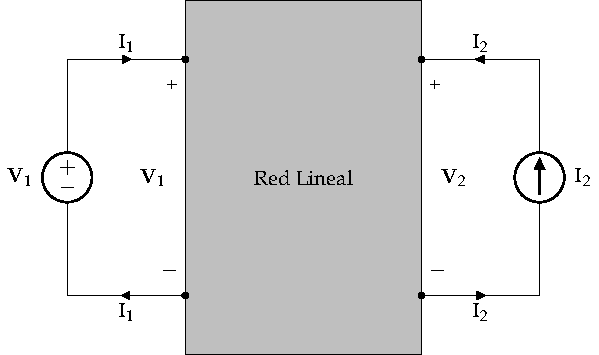
\includegraphics[height=4cm]{../figs/cuadripolo_hibrido_inverso.pdf}
\end{center}

\[
  \left[
    \begin{array}{c}
      \mathbf{I}_1\\
      \mathbf{V}_2
    \end{array}
  \right] =
  \left[
    \begin{array}{cc}
      \mathbf{g}_{11} & \mathbf{g}_{12}\\
      \mathbf{g}_{21} & \mathbf{g}_{22}
    \end{array}
  \right] \cdot
  \left[
    \begin{array}{c}
      \mathbf{V}_1\\
      \mathbf{I}_2
    \end{array}
  \right]
\]

\subsubsection{Circuito Equivalente}
\label{sec:orga0eb94b}
\begin{center}
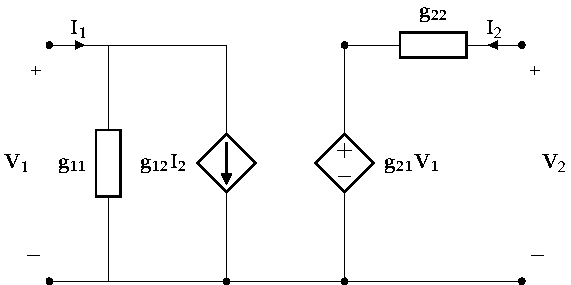
\includegraphics[height=4cm]{../figs/circuitoEquivalenteG.pdf}
\end{center}

\[
\begin{array}{l}
  \mathbf{I}_1 = \mathbf{g}_{11} \mathbf{V}_1 + \mathbf{g}_{12} \mathbf{I}_2\\
  \mathbf{V}_2 = \mathbf{g}_{21} \mathbf{V}_1 + \mathbf{g}_{22} \mathbf{I}_2\\
\end{array}
\]

\subsubsection{Cálculo de parámetros}
\label{sec:org2365b60}

\begin{enumerate}
\item Salida en abierto
\label{sec:org490be28}

\begin{enumerate}
\item \hfill{}\textsc{BMCOL}
\label{sec:orgb210ca2}
\renewcommand{\arraystretch}{2}
\[
  \begin{array}{c}
    \mathbf{g}_{11} = \left.\frac{\mathbf{I}_1}{\mathbf{V}_1}\right\rvert_{\mathbf{I}_2 = 0} \\
    \mathbf{g}_{21} = \left.\frac{\mathbf{V}_2}{\mathbf{V}_1}\right\rvert_{\mathbf{I}_2 = 0}
  \end{array}
\]

\item \hfill{}\textsc{BMCOL}
\label{sec:orga9cc93f}
\begin{center}
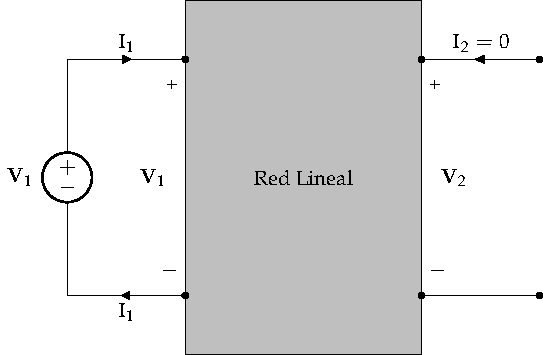
\includegraphics[height=4cm]{../figs/parametrosG_entrada.pdf}
\end{center}
\end{enumerate}

\item \hfill{}\textsc{B\_ignoreheading}
\label{sec:org1c0c522}
\[
  \left[
    \begin{array}{c}
      \mathbf{I}_1\\
      \mathbf{V}_2
    \end{array}
  \right] =
  \left[
    \begin{array}{cc}
      \color{blue}{\mathbf{g}_{11}} & \mathbf{g}_{12}\\
      \color{blue}{\mathbf{g}_{21}} & \mathbf{g}_{22}
    \end{array}
  \right] \cdot
  \left[
    \begin{array}{c}
      \color{blue}{\mathbf{V}_1}\\
      \mathbf{I}_2
    \end{array}
  \right]
\]
\end{enumerate}

\subsubsection{Cálculo de parámetros}
\label{sec:org4b6c520}

\begin{enumerate}
\item Entrada en cortocircuito
\label{sec:org5a8ad67}

\begin{enumerate}
\item \hfill{}\textsc{BMCOL}
\label{sec:org71212cd}
\begin{center}
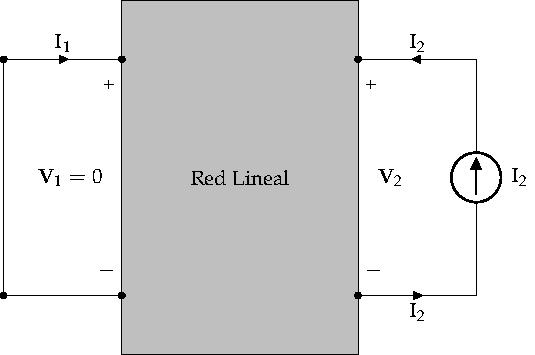
\includegraphics[height=4cm]{../figs/parametrosG_salida.pdf}
\end{center}

\item \hfill{}\textsc{BMCOL}
\label{sec:org0f2ee52}
\renewcommand{\arraystretch}{2}
\[
  \begin{array}{c}
    \mathbf{g}_{12} = \left.\frac{\mathbf{I}_1}{\mathbf{I}_2}\right\rvert_{\mathbf{V}_1 = 0}\\
    \mathbf{g}_{22} = \left.\frac{\mathbf{V}_2}{\mathbf{I}_2}\right\rvert_{\mathbf{V}_1 = 0}
  \end{array}
\]
\end{enumerate}

\item \hfill{}\textsc{B\_ignoreheading}
\label{sec:org5b626bc}
\[
  \left[
    \begin{array}{c}
      \mathbf{I}_1\\
      \mathbf{V}_2
    \end{array}
  \right] =
  \left[
    \begin{array}{cc}
      \mathbf{g}_{11} & \color{blue}{\mathbf{g}_{12}}\\
      \mathbf{g}_{21} & \color{blue}{\mathbf{g}_{22}}
    \end{array}
  \right] \cdot
  \left[
    \begin{array}{c}
      \mathbf{V}_1\\
      \color{blue}{\mathbf{I}_2}
    \end{array}
  \right]
\]
\end{enumerate}


\subsection{Parámetros de Transmisión}
\label{sec:orgd5598b8}

\subsubsection{Definición}
\label{sec:orgcd755d3}
\begin{center}
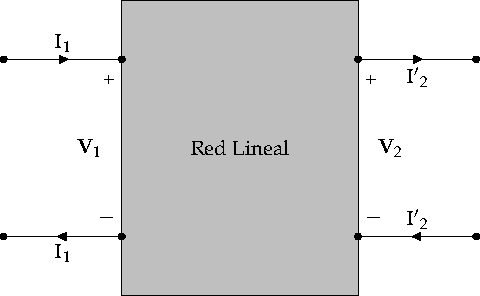
\includegraphics[height=4cm]{../figs/cuadripolo_transmision.pdf}
\end{center}

\[
\begin{array}{l}
  \mathbf{V}_1 = \mathbf{A} \mathbf{V}_2 + \mathbf{B}\mathbf{I'}_2\\
  \mathbf{I}_1 = \mathbf{C} \mathbf{V}_2 + \mathbf{D} \mathbf{I'}_2\\
\end{array}
\]

\begin{center}
\textbf{Atención} al sentido de la corriente \(\mathbf{I'}_2\). (\(\mathbf{I'}_2 = - \mathbf{I}_2\)).
\end{center}

\subsubsection{Expresión Matricial}
\label{sec:org104daf9}
\begin{center}
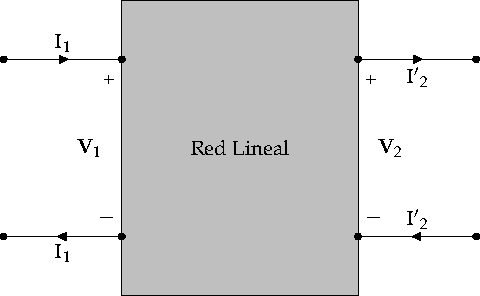
\includegraphics[height=4cm]{../figs/cuadripolo_transmision.pdf}
\end{center}

\[
  \left[
    \begin{array}{c}
      \mathbf{V}_1\\
      \mathbf{I}_1
    \end{array}
  \right] =
  \left[
    \begin{array}{cc}
      \mathbf{A} & \mathbf{B}\\
      \mathbf{C} & \mathbf{D}
    \end{array}
  \right] \cdot
  \left[
    \begin{array}{c}
      \mathbf{V}_2\\
      \mathbf{I'}_2
    \end{array}
  \right]
\]

\subsubsection{Cálculo de parámetros}
\label{sec:org99ce061}

Se debe medir el inverso de cada parámetro, dado que la magnitud a medir y la excitación pertenecen al mismo puerto.

\renewcommand{\arraystretch}{3}
\[
  \begin{array}{cc}
    \frac{1}{\mathbf{A}} = \left.\frac{\mathbf{V}_2}{\mathbf{V}_1}\right\rvert_{\mathbf{I}_2 = 0} &
    \frac{1}{\mathbf{B}} = \left.\frac{\mathbf{I'}_2}{\mathbf{V}_1}\right\rvert_{\mathbf{V}_2 = 0}\\
    \frac{1}{\mathbf{C}} = \left.\frac{\mathbf{V}_2}{\mathbf{I}_1}\right\rvert_{\mathbf{I}_2 = 0} &
    \frac{1}{\mathbf{D}} = \left.\frac{\mathbf{I'}_2}{\mathbf{I}_1}\right\rvert_{\mathbf{V}_2 = 0}\\
  \end{array}
\]

\begin{enumerate}
\item \hfill{}\textsc{BMCOL}
\label{sec:orga42aeb3}
\begin{center}
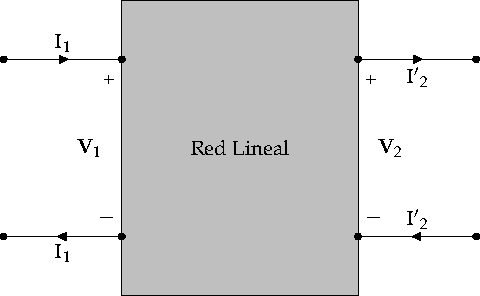
\includegraphics[height=4cm]{../figs/cuadripolo_transmision.pdf}
\end{center}

\item \hfill{}\textsc{BMCOL}
\label{sec:orgb82d084}
\renewcommand{\arraystretch}{1}
\[
\begin{array}{l}
  \mathbf{V}_1 = \mathbf{A} \mathbf{V}_2 + \mathbf{B}\mathbf{I'}_2\\
  \mathbf{I}_1 = \mathbf{C} \mathbf{V}_2 + \mathbf{D} \mathbf{I'}_2\\
\end{array}
\]
\end{enumerate}


\subsection{Parámetros de Transmisión Inversa}
\label{sec:orgd62a71b}

\subsubsection{Definición}
\label{sec:org52b179c}
\begin{center}
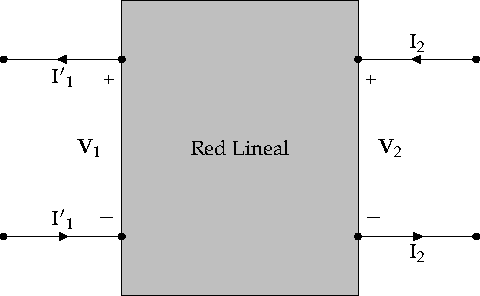
\includegraphics[height=4cm]{../figs/cuadripolo_transmision_inversa.pdf}
\end{center}

\[
\begin{array}{l}
  \mathbf{V}_2 = \mathbf{a} \mathbf{V}_1 + \mathbf{b}\mathbf{I'}_1\\
  \mathbf{I}_2 = \mathbf{c} \mathbf{V}_1 + \mathbf{d} \mathbf{I'}_1\\
\end{array}
\]

\begin{center}
\textbf{Atención} al sentido de la corriente \(\mathbf{I'}_1\) (\(\mathbf{I'}_1 = - \mathbf{I}_1\)).
\end{center}

\subsubsection{Expresión Matricial}
\label{sec:orgca7fb03}
\begin{center}
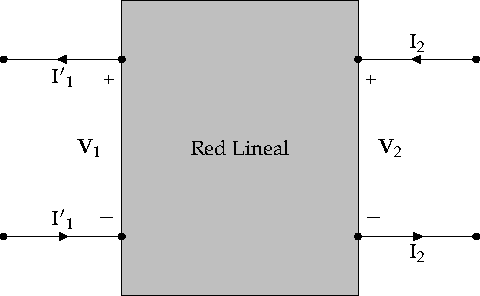
\includegraphics[height=4cm]{../figs/cuadripolo_transmision_inversa.pdf}
\end{center}

\[
  \left[
    \begin{array}{c}
      \mathbf{V}_2\\
      \mathbf{I}_2
    \end{array}
  \right] =
  \left[
    \begin{array}{cc}
      \mathbf{a} & \mathbf{b}\\
      \mathbf{c} & \mathbf{d}
    \end{array}
  \right] \cdot
  \left[
    \begin{array}{c}
      \mathbf{V}_1\\
      \mathbf{I'}_1
    \end{array}
  \right]
\]

\subsubsection{Cálculo de parámetros}
\label{sec:org67b01c0}
Se debe medir el inverso de cada parámetro, dado que la magnitud a medir y la excitación pertenecen al mismo puerto.

\renewcommand{\arraystretch}{3}
\[
  \begin{array}{cc}
    \frac{1}{\mathbf{a}} = \left.\frac{\mathbf{V}_1}{\mathbf{V}_2}\right\rvert_{\mathbf{I}_1 = 0} &
    \frac{1}{\mathbf{b}} = \left.\frac{\mathbf{I'}_1}{\mathbf{V}_2}\right\rvert_{\mathbf{V}_1 = 0}\\
    \frac{1}{\mathbf{c}} = \left.\frac{\mathbf{V}_1}{\mathbf{I}_2}\right\rvert_{\mathbf{I}_1 = 0} &
    \frac{1}{\mathbf{d}} = \left.\frac{\mathbf{I'}_1}{\mathbf{I}_2}\right\rvert_{\mathbf{V}_1 = 0}\\
  \end{array}
\]

\begin{enumerate}
\item \hfill{}\textsc{BMCOL}
\label{sec:org770263e}
\begin{center}
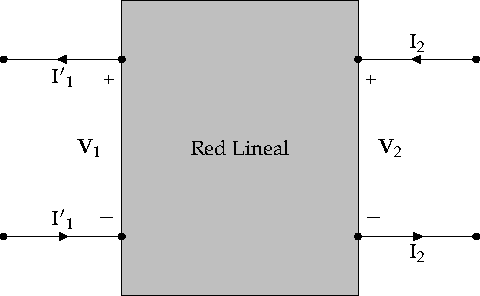
\includegraphics[height=4cm]{../figs/cuadripolo_transmision_inversa.pdf}
\end{center}

\item \hfill{}\textsc{BMCOL}
\label{sec:orgc57f0bc}
\renewcommand{\arraystretch}{1}
\[
\begin{array}{l}
  \mathbf{V}_2 = \mathbf{a} \mathbf{V}_1 + \mathbf{b}\mathbf{I'}_1\\
  \mathbf{I}_2 = \mathbf{c} \mathbf{V}_1 + \mathbf{d} \mathbf{I'}_1\\
\end{array}
\]
\end{enumerate}


\section{Relación entre parámetros}
\label{sec:org2eae33c}

\subsubsection{Impedancia y Admitancia}
\label{sec:orgf5948b7}
\[
  \left.
    \begin{array}{l}
      \left[
      \begin{array}{c}
        \mathbf{V}_1\\
        \mathbf{V}_2
      \end{array}
      \right] =
      \left[
      \begin{array}{cc}
        \mathbf{z}_{11} & \mathbf{z}_{12}\\
        \mathbf{z}_{21} & \mathbf{z}_{22}
      \end{array}
                          \right]
                          \cdot
                          \left[
                          \begin{array}{c}
                            \mathbf{I}_1\\
                            \mathbf{I}_2
                          \end{array}
      \right] \\ \\
      \left[
      \begin{array}{c}
        \mathbf{I}_1\\
        \mathbf{I}_2
      \end{array}
      \right] =
      \left[
      \begin{array}{cc}
        \mathbf{y}_{11} & \mathbf{y}_{12}\\
        \mathbf{y}_{21} & \mathbf{y}_{22}
      \end{array}
                          \right] \cdot
                          \left[
                          \begin{array}{c}
                            \mathbf{V}_1\\
                            \mathbf{V}_2
                          \end{array}
      \right]
    \end{array}
    \right\}
      \rightarrow
      \boxed{[\mathbf{Z}] = [\mathbf{Y}]^{-1}}
    \]

\subsubsection{Híbridos}
\label{sec:org34b878b}
\[
  \left.
    \begin{array}{l}
      %% Híbridos
  \left[
    \begin{array}{c}
      \mathbf{V}_1\\
      \mathbf{I}_2
    \end{array}
  \right] =
  \left[
    \begin{array}{cc}
      \mathbf{h}_{11} & \mathbf{h}_{12}\\
      \mathbf{h}_{21} & \mathbf{h}_{22}
    \end{array}
  \right] \cdot
  \left[
    \begin{array}{c}
      \mathbf{I}_1\\
      \mathbf{V}_2
    \end{array}
      \right]
      \\ \\
      %% Híbridos Inversos
  \left[
    \begin{array}{c}
      \mathbf{I}_1\\
      \mathbf{V}_2
    \end{array}
  \right] =
  \left[
    \begin{array}{cc}
      \mathbf{g}_{11} & \mathbf{g}_{12}\\
      \mathbf{g}_{21} & \mathbf{g}_{22}
    \end{array}
  \right] \cdot
  \left[
    \begin{array}{c}
      \mathbf{V}_1\\
      \mathbf{I}_2
    \end{array}
      \right]
      \end{array}
    \right\}
      \rightarrow
      \boxed{[\mathbf{H}] = [\mathbf{G}]^{-1}}
    \]
\subsubsection{Transmisión}
\label{sec:org47212d8}
\[
  \left.
    \begin{array}{l}
      %% Transmisión
  \left[
    \begin{array}{c}
      \mathbf{V}_1\\
      \mathbf{I}_1
    \end{array}
  \right] =
  \left[
    \begin{array}{cc}
      \mathbf{A} & \mathbf{B}\\
      \mathbf{C} & \mathbf{D}
    \end{array}
  \right] \cdot
  \left[
    \begin{array}{c}
      \mathbf{V}_2\\
      \mathbf{I'}_2
    \end{array}
  \right]
      \\ \\
      %% Transmisión Inversa
  \left[
    \begin{array}{c}
      \mathbf{V}_2\\
      \mathbf{I}_2
    \end{array}
  \right] =
  \left[
    \begin{array}{cc}
      \mathbf{a} & \mathbf{b}\\
      \mathbf{c} & \mathbf{d}
    \end{array}
  \right] \cdot
  \left[
    \begin{array}{c}
      \mathbf{V}_1\\
      \mathbf{I'}_1
    \end{array}
  \right]
      \end{array}
    \right\}
    \rightarrow
    \boxed{[\mathbf{T}] \neq [\mathbf{t}]^{-1}}
  \]
\[
  \boxed{
    \left[
      \begin{array}{cc}
        \mathbf{A} & \mathbf{B}\\
        \mathbf{C} & \mathbf{D}
      \end{array}\right] = 
      \left[
      \begin{array}{cc}
        \mathbf{a} & \mathbf{-b}\\
        \mathbf{-c} & \mathbf{d}
      \end{array}
      \right]^{-1}
    }
\]
\subsubsection{}
\label{sec:orgf3da70f}
\begin{center}
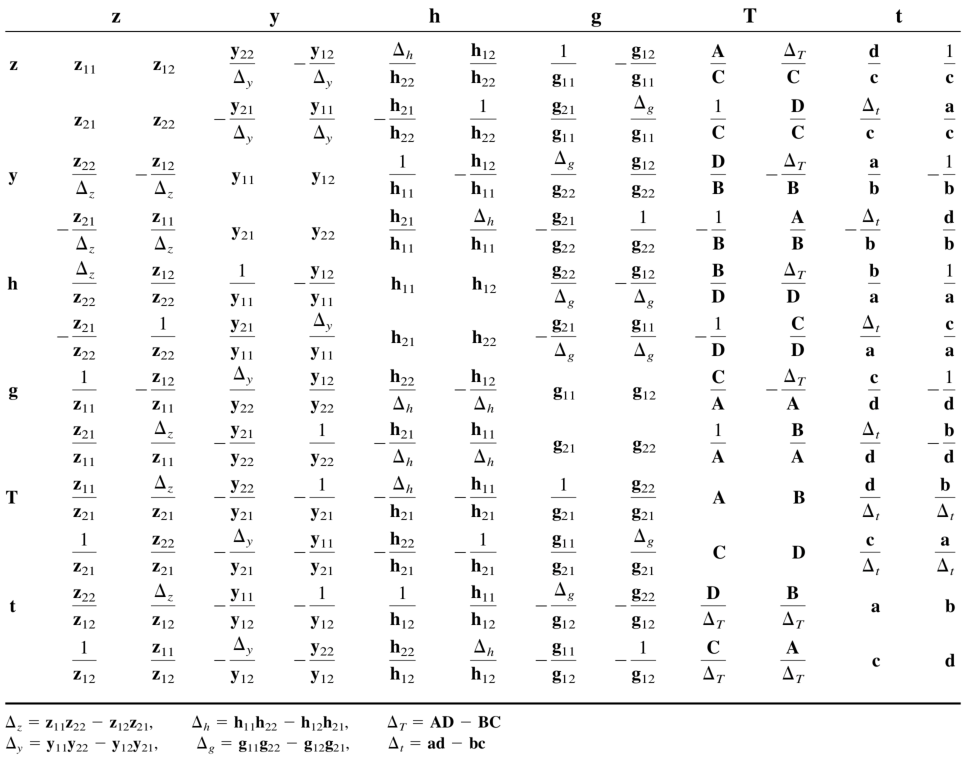
\includegraphics[height=4cm]{../figs/Tabla_Parametros.pdf}
\end{center}

\subsubsection{Reciprocidad}
\label{sec:org8de0a87}
A partir de las relaciones ya obtenidas para impedancia y admitancia, utilizando la tabla anterior obtenemos la relación para parámetros híbridos y de transmisión:
\[
\left.
\begin{array}{l}
  \mathbf{z_{12}} = \mathbf{z_{21}}\\
  \mathbf{y_{12}} = \mathbf{y_{21}}\\
\end{array}
\right\} \rightarrow
\left\{
\begin{array}{l}
  \mathbf{h_{12}} = - \mathbf{h_{21}}\\
  \mathbf{g_{12}} = - \mathbf{g_{21}}\\
  \mathbf{A} \mathbf{D} - \mathbf{B} \mathbf{C} = 1\\
  \mathbf{a} \mathbf{d} - \mathbf{b} \mathbf{c} = 1\\
\end{array}
\right.
\]


\subsubsection{Simetría}
\label{sec:org32ff848}
A partir de las relaciones ya obtenidas para impedancia y admitancia, utilizando la tabla anterior obtenemos la relación para parámetros híbridos y de transmisión:
\[
\left.
\begin{array}{l}
  \mathbf{z_{11}} = \mathbf{z_{22}}\\
  \mathbf{y_{11}} = \mathbf{y_{22}}\\
\end{array}
\right\} \rightarrow
\left\{
\begin{array}{l}
  \mathbf{h_{11}} \cdot \mathbf{h_{22}} - \mathbf{h_{12}}^2 = 1\\
  \mathbf{g_{11}} \cdot \mathbf{g_{22}} - \mathbf{g_{12}}^2 = 1\\
  \mathbf{A} =  \mathbf{D}\\
  \mathbf{a} =  \mathbf{d}\\
\end{array}
\right.
\]

Además:

\[
  \boxed{[\mathbf{T}] = [\mathbf{t}]}
\]


\section{Cuadripolos entre Dipolos Terminales}
\label{sec:org4eb70ca}

\subsection{Situación General}
\label{sec:orgf52f6e2}
\subsubsection{}
\label{sec:org495ece7}
\begin{center}
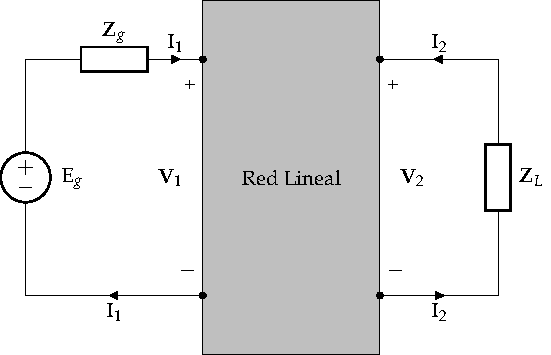
\includegraphics[height=4cm]{../figs/cuadripolo_cargado_fuente_tension.pdf}
\end{center}

\begin{align*}
  \mathbf{V}_1 &= \mathbf{E}_g - \mathbf{Z}_g \cdot \mathbf{I}_1\\
  \mathbf{V}_2 &= - \mathbf{Z}_L \cdot \mathbf{I}_2\\
\end{align*}

\subsubsection{}
\label{sec:orgc9420fa}
\begin{center}
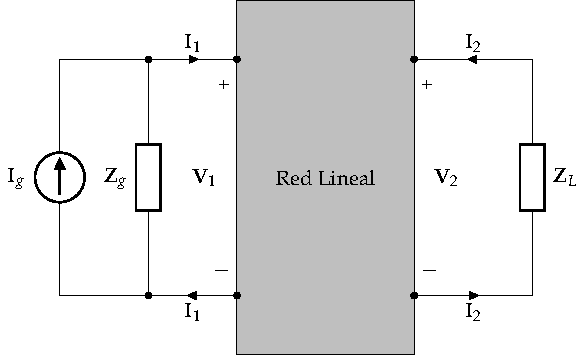
\includegraphics[height=4cm]{../figs/cuadripolo_cargado_fuente_corriente.pdf}
\end{center}

\begin{align*}
  \mathbf{V}_1 &= (\mathbf{I}_g - \mathbf{I}_1) \cdot \mathbf{Z}_g\\
  \mathbf{V}_2 &= - \mathbf{Z}_L \cdot \mathbf{I}_2\\
\end{align*}

\subsubsection{Ganancia}
\label{sec:orge1f4b88}

\begin{enumerate}
\item \hfill{}\textsc{BMCOL}
\label{sec:org1a393ee}
\begin{center}
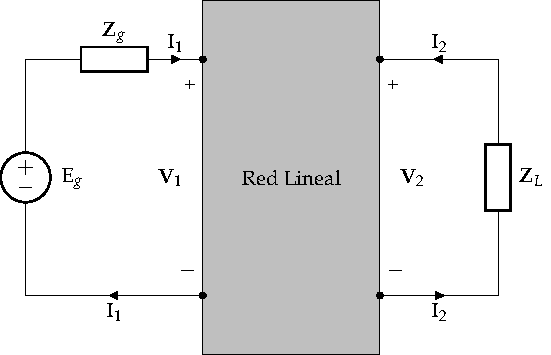
\includegraphics[height=4cm]{../figs/cuadripolo_cargado_fuente_tension.pdf}
\end{center}
\begin{center}
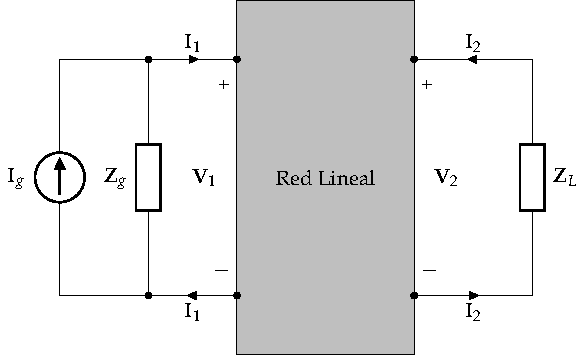
\includegraphics[height=4cm]{../figs/cuadripolo_cargado_fuente_corriente.pdf}
\end{center}


\item \hfill{}\textsc{BMCOL}
\label{sec:org77ac402}
\begin{itemize}
\item Ganancia de Tensión
\end{itemize}
\[
\mathbf{A}_V = \frac{\mathbf{V}_2}{\mathbf{E}_g}
\]
\begin{itemize}
\item Ganancia de Corriente
\end{itemize}
\[
\mathbf{A}_I = \frac{\mathbf{I}_2}{\mathbf{I}_g}
\]
\end{enumerate}

\subsubsection{Impedancia}
\label{sec:org591ea39}
\begin{enumerate}
\item \hfill{}\textsc{BMCOL}
\label{sec:orgd9d6752}
\begin{center}
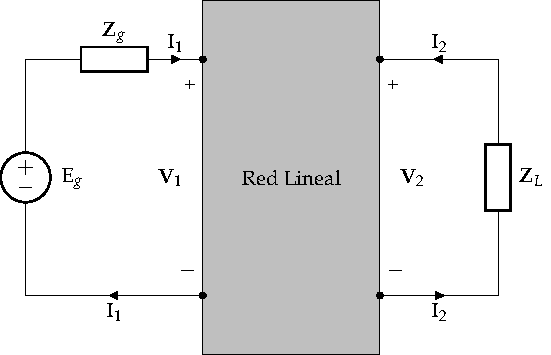
\includegraphics[height=4cm]{../figs/cuadripolo_cargado_fuente_tension.pdf}
\end{center}
\begin{center}
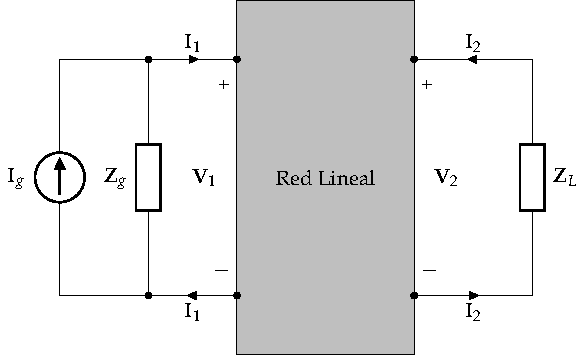
\includegraphics[height=4cm]{../figs/cuadripolo_cargado_fuente_corriente.pdf}
\end{center}


\item \hfill{}\textsc{BMCOL}
\label{sec:orgc27df88}
\begin{itemize}
\item Impedancia de Entrada
\end{itemize}
\[
\mathbf{Z}_i = \frac{\mathbf{V}_1}{\mathbf{I}_1}
\]

\begin{itemize}
\item Impedancia de Salida
\end{itemize}
\[
\mathbf{Z}_o = \left.\frac{\mathbf{V}_2}{\mathbf{I}_2}\right\rvert_{\mathbf{E}_g = 0}
\]
\end{enumerate}

\subsubsection{Transferencia}
\label{sec:orgb5d33e6}
\begin{enumerate}
\item \hfill{}\textsc{BMCOL}
\label{sec:org6258e98}
\begin{center}
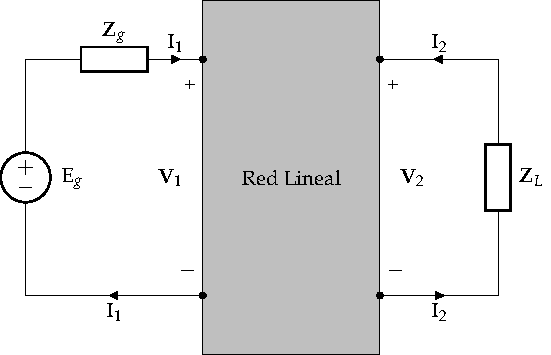
\includegraphics[height=4cm]{../figs/cuadripolo_cargado_fuente_tension.pdf}
\end{center}
\begin{center}
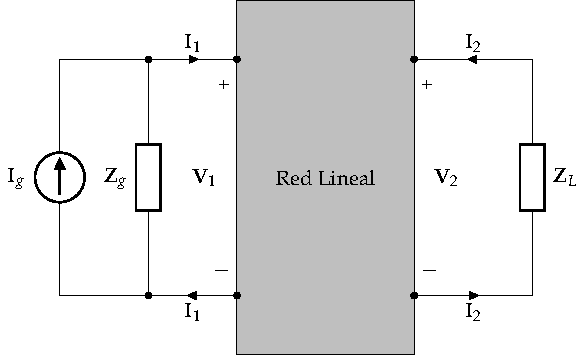
\includegraphics[height=4cm]{../figs/cuadripolo_cargado_fuente_corriente.pdf}
\end{center}


\item \hfill{}\textsc{BMCOL}
\label{sec:org8c9bbdc}
\begin{itemize}
\item Transadmitancia directa
\end{itemize}
\[
\mathbf{Y}_f = \frac{\mathbf{I}_2}{\mathbf{E}_g}
\]

\begin{itemize}
\item Transimpedancia directa
\end{itemize}
\[
\mathbf{Z}_f = \frac{\mathbf{V}_2}{\mathbf{I}_g}
\]
\end{enumerate}

\subsubsection{Ejercicio de Cálculo (1)}
\label{sec:orgce5d563}

Demuestra que la impedancia de entrada del circuito a la derecha de la fuente real expresada con parámetros de transmisión es:

\[
\mathbf{Z}_i = \frac{\mathbf{A} \mathbf{Z}_L + \mathbf{B}}{\mathbf{C}\mathbf{Z}_L + \mathbf{D}}
\]

\begin{center}
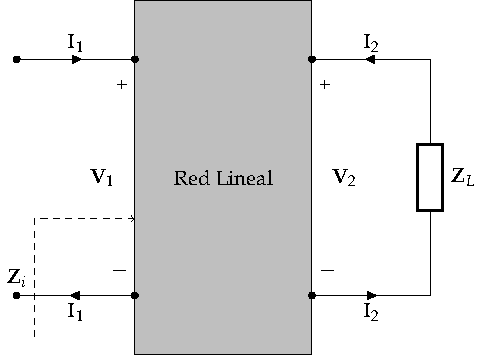
\includegraphics[height=4cm]{../figs/cuadripolo_cargado_impedancia_entrada.pdf}
\end{center}



\subsubsection{Ejercicio de Cálculo (2)}
\label{sec:org2e2860e}

¿Qué impedancia de carga \(\mathbf{Z}_L\) hay que conectar a la salida del cuadripolo para obtener la máxima transferencia de potencia?

\begin{center}
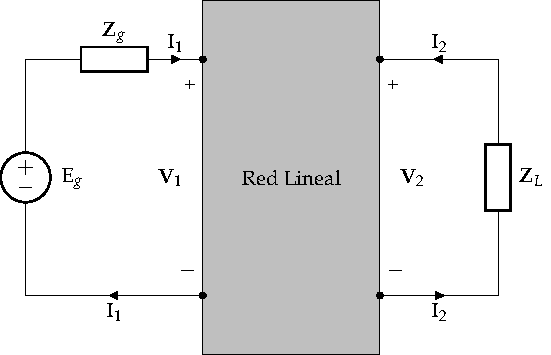
\includegraphics[height=4cm]{../figs/cuadripolo_cargado_fuente_tension.pdf}
\end{center}

\subsection{Parámetros Imagen}
\label{sec:org5e458cf}

\subsubsection{Impedancia Característica}
\label{sec:orgcd34bb0}
Para un cuadripolo \textbf{recíproco} y \textbf{simétrico} se definen los parámetros imagen:

\begin{itemize}
\item \textbf{Impedancia característica}, \(\mathbf{Z}_o\): impedancia que, conectada en una puerta, hace que desde la otra puerta se vea la misma impedancia.
\end{itemize}
\[
  \mathbf{Z}_o = \frac{\mathbf{U}_1}{\mathbf{I}_1}
\]

\begin{enumerate}
\item \hfill{}\textsc{BMCOL}
\label{sec:org302b662}
\begin{center}
\includegraphics[height=4cm]{../figs/cuadripolo_impedancia_caracteristica.pdf}
\end{center}

\item \hfill{}\textsc{BMCOL}
\label{sec:orgc75359e}
\[
\mathbf{Z}_o = \frac{\mathbf{A} \mathbf{Z}_o + \mathbf{B}}{\mathbf{C}\mathbf{Z}_o + \mathbf{D}}
\]

\[
\mathbf{A} = \mathbf{D} \rightarrow \boxed{\mathbf{Z}_o = \pm \sqrt{\frac{\mathbf{B}}{\mathbf{C}}}}
\]
\end{enumerate}

\subsubsection{Impedancia Característica}
\label{sec:org7144bfc}

\begin{enumerate}
\item Atención
\label{sec:org9042c98}
La ecuación proporciona dos soluciones, una de las cuáles implicará una impedancia no viable (\emph{resistencia negativa}).
\[
\boxed{\mathbf{Z}_o = \pm \sqrt{\frac{\mathbf{B}}{\mathbf{C}}}}
\]
\end{enumerate}

\subsubsection{Función de Propagación}
\label{sec:orgf2ef1cc}
Para un cuadripolo \textbf{recíproco} y \textbf{simétrico} se definen los parámetros imagen:

\begin{itemize}
\item \textbf{Función de propagación}, \(\gamma\): relacionada con el cociente de potencias en las puertas del cuadripolo cuando una de ellas está cargada con \(\mathbf{Z}_o\)
\end{itemize}

\[
  \exp(2\gamma) = \frac{\mathbf{U}_1\mathbf{I}_1}{\mathbf{U}_2\mathbf{I}'_2}
\]

\begin{enumerate}
\item \hfill{}\textsc{BMCOL}
\label{sec:org884522a}
\begin{center}
\includegraphics[height=4cm]{../figs/cuadripolo_impedancia_caracteristica.pdf}
\end{center}

\item \hfill{}\textsc{BMCOL}
\label{sec:org13d5d40}
\begin{align*}
  \mathbf{U}_1 &= \mathbf{I}_1 \mathbf{Z}_o\\
  \mathbf{U}_2 &= \mathbf{I}'_2 \mathbf{Z}_o
\end{align*}

\[
  \boxed{\exp(\gamma) = \frac{\mathbf{U}_1}{\mathbf{U}_2} = \frac{\mathbf{I}_1}{\mathbf{I}'_2}}
\]
\end{enumerate}


\subsubsection{Relación entre \(\mathbf{Z}_o\) y \(\gamma\)}
\label{sec:orgba47dd9}
\begin{enumerate}
\item \hfill{}\textsc{BMCOL}
\label{sec:org93db8e6}
\begin{center}
\includegraphics[height=4cm]{../figs/cuadripolo_impedancia_caracteristica.pdf}
\end{center}

\item \hfill{}\textsc{BMCOL}
\label{sec:org51048e6}
\begin{align*}
  \exp(\gamma) &= \frac{\mathbf{U}_1}{\mathbf{U}_2} =\\
               &= \frac{\mathbf{A}\mathbf{U}_2 + \mathbf{B}\mathbf{I}'_2}{\mathbf{U}_2} = \\
               &= \mathbf{A} + \mathbf{B}\frac{\mathbf{I}'_2}{\mathbf{U_2}}
\end{align*}

\[
  \boxed{\exp(\gamma) = \mathbf{A} + \frac{\mathbf{B}}{\mathbf{Z}_o}}
\]
\end{enumerate}

\subsubsection{Relación entre \(\mathbf{Z}_o\) y \(\gamma\)}
\label{sec:org2783cff}

Teniendo en cuenta la expresión de \(\mathbf{Z}_o\):
\[
  \left.
  \begin{array}{l}
    \mathbf{Z}_o = \pm \sqrt{\frac{\mathbf{B}}{\mathbf{C}}}\\
    \exp(\gamma) = \mathbf{A} + \frac{\mathbf{B}}{\mathbf{Z}_o}
  \end{array} \right\} \rightarrow
\boxed{\exp(\gamma) = \mathbf{A} \pm \sqrt{\mathbf{B}\mathbf{C}}}
\]

Además, teniendo en cuenta la relación de un cuadripolo recíproco y simétrico:

\[
  \mathbf{A}^2 - \mathbf{B}\mathbf{C} = 1 \rightarrow %
  \boxed{\exp(\gamma) = \mathbf{A} \pm \sqrt{\mathbf{A}^2 - 1}}
\]
\textbf{Atención} al signo que acompaña a las raíces cuadradas. Se debe elegir de forma que la parte real de \(\gamma\) sea acorde al cuadripolo.

\subsubsection{Transmisión a partir de Imagen}
\label{sec:org593cab5}

\[
\mathbf{A}^2 - \mathbf{B}\mathbf{C} = 1
\]

\begin{enumerate}
\item \hfill{}\textsc{BMCOL}
\label{sec:orgbfdda51}
\[
  e^\gamma = \mathbf{A} + \sqrt{\mathbf{A}^2 - 1}
\]

\[
  \mathbf{Z}_o = \sqrt{\frac{\mathbf{B}}{\mathbf{C}}}
\]

\item \hfill{}\textsc{BMCOL}
\label{sec:orgbb55298}
\begin{align*}
  \cosh(\gamma) &= \frac{e^\gamma + e^{-\gamma}}{2}\\
  \sinh(\gamma) &= \frac{e^\gamma - e^{-\gamma}}{2}\\
  \cosh^2(\gamma) &- \sinh^2(\gamma) = 1
\end{align*}

\item \hfill{}\textsc{B\_ignoreheading}
\label{sec:org51374bf}
\[
\boxed{
  \begin{array}{ll}
    \mathbf{A} = \cosh(\gamma) &
    \mathbf{B} = \mathbf{Z}_o \sinh(\gamma)\\
    \mathbf{C} = \sinh(\gamma)/\mathbf{Z}_o &
    \mathbf{D} = \cosh(\gamma)\\
  \end{array}
}
\]
\end{enumerate}

\subsubsection{Régimen Permanente Sinusoidal}
\label{sec:orgde43a7b}

Cuando el circuito funciona en régimen permanente sinusoidal:

\begin{itemize}
\item La función de propagación es un número complejo denominado constante de propagación.
\end{itemize}
\[
  \overline{\gamma} = \alpha + j\beta
\]
\begin{itemize}
\item Las tensiones y corrientes son fasores
\end{itemize}
\[
  \exp(\overline{\gamma}) = \exp(\alpha) \cdot \exp(j\beta) = \frac{\overline{U}_1}{\overline{U}_2} = \frac{\overline{I}_1}{\overline{I}'_2}
\]

\subsubsection{Régimen Permanente Sinusoidal}
\label{sec:org6afeb0f}
\begin{itemize}
\item \textbf{Constante de Atenuación} (cuando \(\alpha > 1\) el cuadripolo atenúa la salida respecto de la entrada)
\end{itemize}
\[
  \exp(\alpha) = \frac{U_1}{U_2} = \frac{I_1}{I_2}
\]
\begin{itemize}
\item \textbf{Constante de Fase} (desfase entre puertos)
\end{itemize}
\[
  \beta = \theta_{\overline{U}_1} - \theta_{\overline{U}_2} = \theta_{\overline{I}_1} - \theta_{\overline{I}'_2}
\]

\subsubsection{Atenuación de Potencia}
\label{sec:org3c1bb07}

\textbf{Cuando está conectada la impedancia característica}, las potencias activas en los puertos se expresan:

\begin{align*}
  P_1 &= U_1 I_1 \cos(\theta_o)\\
  P_2 &= U_2 I_2 \cos(\theta_o)
\end{align*}
donde \(\theta_o\) es el ángulo de la impedancia \(\overline{Z}_o\).

Por tanto, la relación de potencias activas es:

\[
\frac{P_1}{P_2} = \frac{U_1 I_1}{U_2 I_2}
\]
Teniendo en cuenta la expresión de la constante de atenuación, esta relación es:
\[
    \exp(\alpha) = \frac{U_1}{U_2} = \frac{I_1}{I_2} \rightarrow \boxed{\exp(2\alpha) = \frac{U_1 I_1}{U_2 I_1} = \frac{P_1}{P_2}}
\]

\section{Asociación de Cuadripolos}
\label{sec:org69d0c87}

\subsubsection{Conexiones}
\label{sec:orgf6e2051}

\begin{enumerate}
\item Definición
\label{sec:org531ded7}
\begin{itemize}
\item \textbf{Serie}: misma corriente, suma de tensiones
\item \textbf{Paralelo}: misma tensión, suma de corrientes
\end{itemize}
\item Catálogo
\label{sec:org94028dc}
\begin{itemize}
\item Serie-Serie: \textbf{parámetros impedancia}
\item Paralelo-Paralelo: \textbf{parámetros admitancia}
\item Serie-Paralelo: \textbf{parámetros híbridos}
\item Paralelo-Serie: \textbf{parámetros híbridos inversos}
\item Cascada: \textbf{parámetros transmisión/imagen}
\end{itemize}
\end{enumerate}
\subsection{Asociación Serie-Serie}
\label{sec:orgf8c64c4}

\subsubsection{Conexión}
\label{sec:org93220a5}

\begin{enumerate}
\item \hfill{}\textsc{BMCOL}
\label{sec:orgfbc403e}
\begin{center}
\includegraphics[height=4cm]{../figs/serie-serie.pdf}
\end{center}



\item \hfill{}\textsc{BMCOL}
\label{sec:orgb817874}
\begin{enumerate}
\item Tensiones
\label{sec:orgbdd8729}
\begin{align*}
  \mathbf{V}_1 &= \mathbf{V}_{1A} + \mathbf{V}_{1B}\\
  \mathbf{V}_2 &= \mathbf{V}_{2A} + \mathbf{V}_{2B}
\end{align*}

\item Condición de Puerto
\label{sec:org70529d0}
\begin{align*}
  \mathbf{I}_{1A} &= \mathbf{I}_{1'A}\\
  \mathbf{I}_{1B} &= \mathbf{I}_{1'B}\\
  \mathbf{I}_{2A} &= \mathbf{I}_{2'A}\\
  \mathbf{I}_{2B} &= \mathbf{I}_{2'B}
\end{align*}
\end{enumerate}
\end{enumerate}

\subsubsection{Cuadripolo Equivalente}
\label{sec:orga827299}
\begin{enumerate}
\item \hfill{}\textsc{BMCOL}
\label{sec:org213121f}
\begin{center}
\includegraphics[height=4cm]{../figs/serie-serie.pdf}
\end{center}


\item \hfill{}\textsc{BMCOL}
\label{sec:org38dbe81}
\begin{enumerate}
\item Parámetros Impedancia
\label{sec:orgb198b8f}
\begin{align*}
  [\mathbf{V}_A] &= [\mathbf{Z}_A] \cdot [\mathbf{I}_A]\\
  [\mathbf{V}_B] &= [\mathbf{Z}_B] \cdot [\mathbf{I}_B]
\end{align*}

\item Cuadripolo Equivalente
\label{sec:org2696460}
\[
  \boxed{[\mathbf{Z}] = [\mathbf{Z}_A] + [\mathbf{Z}_B]}
\]
\end{enumerate}
\end{enumerate}

\subsubsection{Interacción}
\label{sec:org9daf72f}
\begin{enumerate}
\item \hfill{}\textsc{BMCOL}
\label{sec:orgfd071da}
\begin{center}
\includegraphics[height=5cm]{../figs/serie-serie-interaccion.pdf}
\end{center}
\item \hfill{}\textsc{BMCOL}
\label{sec:org009a6eb}
\begin{itemize}
\item Entrada
\end{itemize}
\begin{align*}
  \mathbf{I}_{1A} &= \mathbf{I}_{g1}\\
  \mathbf{I}_{1'A} &= \mathbf{I}_{g1} - \mathbf{I}_h
\end{align*}
\begin{itemize}
\item Salida
\end{itemize}
\begin{align*}
  \mathbf{I}_{2A} &= \mathbf{I}_{g2}\\
  \mathbf{I}_{2'A} &= \mathbf{I}_{g2}  + \mathbf{I}_h
\end{align*}
\begin{itemize}
\item Condición de Puerto
\end{itemize}
\[
\boxed{\mathbf{I}_h = 0}
\]
\end{enumerate}
\subsubsection{Interacción}
\label{sec:org45b1cf7}
Si no hay interacción, al aplicar superposición la corriente de circulación debe ser nula \textbf{en ambos casos}.
\begin{enumerate}
\item \hfill{}\textsc{BMCOL}
\label{sec:org7b3b505}
\begin{center}
\includegraphics[height=5cm]{../figs/serie-serie-superposicion-entrada.pdf}
\end{center}
\item \hfill{}\textsc{BMCOL}
\label{sec:orgfc7026f}
\begin{center}
\includegraphics[height=5cm]{../figs/serie-serie-superposicion-salida.pdf}
\end{center}
\end{enumerate}

\subsubsection{Test de Brune}
\label{sec:org9a27190}
Aplicando superposición desconectamos los cuadripolos: \textbf{si no hay interacción, no habrá cambio de tensión}.
\begin{enumerate}
\item \hfill{}\textsc{BMCOL}
\label{sec:org3157d40}
\begin{center}
\includegraphics[height=5cm]{../figs/serie-serie-brune-entrada.pdf}
\end{center}
\item \hfill{}\textsc{BMCOL}
\label{sec:org355faf6}
\begin{center}
\includegraphics[height=5cm]{../figs/serie-serie-brune-salida.pdf}
\end{center}
\end{enumerate}


\subsubsection{Métodos para evitar interacción}
\label{sec:org033b270}
\begin{center}
\includegraphics[height=4cm]{../figs/serie-serie-transformador.pdf}
\end{center}

\subsubsection{Métodos para evitar interacción}
\label{sec:org7265967}
\begin{center}
\includegraphics[height=4cm]{../figs/serie-serie-corto.pdf}
\end{center}

\subsection{Asociación Paralelo-Paralelo}
\label{sec:org3afa958}
\subsubsection{Conexión}
\label{sec:org39169d7}
\begin{enumerate}
\item \hfill{}\textsc{BMCOL}
\label{sec:org8edd165}
\begin{center}
\includegraphics[height=4cm]{../figs/paralelo-paralelo.pdf}
\end{center}
\item \hfill{}\textsc{BMCOL}
\label{sec:orgc8c6f3c}
\begin{enumerate}
\item Corrientes
\label{sec:orgb710c53}
\begin{align*}
  \mathbf{I}_1 &= \mathbf{I}_{1A} + \mathbf{I}_{1B}\\
  \mathbf{I}_2 &= \mathbf{I}_{2A} + \mathbf{I}_{2B}
\end{align*}

\item Condición de Puerto
\label{sec:orgf90580b}
\begin{align*}
  \mathbf{I}_{1A} &= \mathbf{I}_{1'A}\\
  \mathbf{I}_{1B} &= \mathbf{I}_{1'B}\\
  \mathbf{I}_{2A} &= \mathbf{I}_{2'A}\\
  \mathbf{I}_{2B} &= \mathbf{I}_{2'B}
\end{align*}
\end{enumerate}
\end{enumerate}

\subsubsection{Cuadripolo Equivalente}
\label{sec:org0bc310b}
\begin{enumerate}
\item \hfill{}\textsc{BMCOL}
\label{sec:org0d6fdf5}
\begin{center}
\includegraphics[height=4cm]{../figs/paralelo-paralelo.pdf}
\end{center}


\item \hfill{}\textsc{BMCOL}
\label{sec:org582370f}
\begin{enumerate}
\item Parámetros Admitancia
\label{sec:org0aeffe8}
\begin{align*}
  [\mathbf{I}_A] &= [\mathbf{Y}_A] \cdot [\mathbf{V}_A]\\
  [\mathbf{I}_B] &= [\mathbf{Y}_B] \cdot [\mathbf{V}_B]
\end{align*}

\item Cuadripolo Equivalente
\label{sec:orgdcc9958}
\[
  \boxed{[\mathbf{Y}] = [\mathbf{Y}_A] + [\mathbf{Y}_B]}
\]
\end{enumerate}
\end{enumerate}
\subsubsection{Interacción}
\label{sec:orgd584cd4}
\begin{center}
\includegraphics[height=4cm]{../figs/paralelo-paralelo-interaccion.pdf}
\end{center}
\subsubsection{Interacción}
\label{sec:orgf1d8a5b}
Si no hay interacción, al aplicar superposición la corriente de circulación debe ser nula \textbf{en ambos casos}.
\begin{enumerate}
\item \hfill{}\textsc{BMCOL}
\label{sec:orgaa86e5c}
\begin{center}
\includegraphics[height=5cm]{../figs/paralelo-paralelo-superposicion-entrada.pdf}
\end{center}
\item \hfill{}\textsc{BMCOL}
\label{sec:org5b95701}
\begin{center}
\includegraphics[height=5cm]{../figs/paralelo-paralelo-superposicion-salida.pdf}
\end{center}
\end{enumerate}

\subsubsection{Test de Brune}
\label{sec:org2591d22}
Aplicando superposición desconectamos los cuadripolos: \textbf{si no hay interacción, no habrá cambio de tensión}.
\begin{enumerate}
\item \hfill{}\textsc{BMCOL}
\label{sec:org951e127}
\begin{center}
\includegraphics[height=5cm]{../figs/paralelo-paralelo-brune-entrada.pdf}
\end{center}
\item \hfill{}\textsc{BMCOL}
\label{sec:orgc2f98c6}
\begin{center}
\includegraphics[height=5cm]{../figs/paralelo-paralelo-brune-salida.pdf}
\end{center}
\end{enumerate}

\subsubsection{Test de Brune}
\label{sec:org199da56}
Aplicando superposición desconectamos los cuadripolos: \textbf{si no hay interacción, no habrá cambio de tensión}.
\begin{enumerate}
\item \hfill{}\textsc{BMCOL}
\label{sec:orge3bd0e3}
\begin{center}
\includegraphics[height=5cm]{../figs/paralelo-paralelo-brune-entrada2.pdf}
\end{center}
\item \hfill{}\textsc{BMCOL}
\label{sec:org745f22c}
\begin{center}
\includegraphics[height=5cm]{../figs/paralelo-paralelo-brune-salida2.pdf}
\end{center}
\end{enumerate}

\subsubsection{Métodos para evitar interacción}
\label{sec:org31cbc7e}
\begin{center}
\includegraphics[height=4cm]{../figs/paralelo-paralelo-transformador.pdf}
\end{center}
\subsubsection{Métodos para evitar interacción}
\label{sec:org3abee48}
\begin{center}
\includegraphics[height=4cm]{../figs/paralelo-paralelo-corto.pdf}
\end{center}
\subsection{Asociación Serie-Paralelo}
\label{sec:orgc44bd68}
\subsubsection{Conexión}
\label{sec:orgcba0d44}
\begin{enumerate}
\item \hfill{}\textsc{BMCOL}
\label{sec:orgb6b388b}
\begin{center}
\includegraphics[height=4cm]{../figs/serie-paralelo.pdf}
\end{center}
\item \hfill{}\textsc{BMCOL}
\label{sec:org547d1ed}
\begin{enumerate}
\item Relaciones
\label{sec:org9cf9c76}
\begin{align*}
  \mathbf{V}_1 &= \mathbf{V}_{1A} + \mathbf{V}_{1B}\\
  \mathbf{I}_2 &= \mathbf{I}_{2A} + \mathbf{I}_{2B}
\end{align*}

\item Cuadripolo Equivalente
\label{sec:orgb751890}
\[
  \boxed{[\mathbf{H}] = [\mathbf{H}_A] + [\mathbf{H}_B]}
\]
\end{enumerate}
\end{enumerate}
\subsubsection{Test de Brune}
\label{sec:orgb1acd8e}
Aplicando superposición desconectamos los cuadripolos: \textbf{si no hay interacción, no habrá cambio de tensión}.
\begin{enumerate}
\item \hfill{}\textsc{BMCOL}
\label{sec:orge70fe59}
\begin{center}
\includegraphics[height=5cm]{../figs/serie-paralelo-brune-entrada.pdf}
\end{center}
\item \hfill{}\textsc{BMCOL}
\label{sec:orgfd2f144}
\begin{center}
\includegraphics[height=5cm]{../figs/serie-paralelo-brune-salida.pdf}
\end{center}
\end{enumerate}

\subsection{Asociación Paralelo-Serie}
\label{sec:orgd91e058}
\subsubsection{Conexión}
\label{sec:org5e14c91}
\begin{enumerate}
\item \hfill{}\textsc{BMCOL}
\label{sec:org43cb61d}
\begin{center}
\includegraphics[height=4cm]{../figs/paralelo-serie.pdf}
\end{center}
\item \hfill{}\textsc{BMCOL}
\label{sec:orge5d2f92}
\begin{enumerate}
\item Relaciones
\label{sec:orge6945d2}
\begin{align*}
  \mathbf{I}_1 &= \mathbf{I}_{1A} + \mathbf{I}_{1B}\\
  \mathbf{V}_2 &= \mathbf{V}_{2A} + \mathbf{V}_{2B}
\end{align*}

\item Cuadripolo Equivalente
\label{sec:orgd5cfc0b}
\[
  \boxed{[\mathbf{G}] = [\mathbf{G}_A] + [\mathbf{G}_B]}
\]
\end{enumerate}
\end{enumerate}

\subsubsection{Test de Brune}
\label{sec:org7667a46}
Aplicando superposición desconectamos los cuadripolos: \textbf{si no hay interacción, no habrá cambio de tensión}.
\begin{enumerate}
\item \hfill{}\textsc{BMCOL}
\label{sec:orga5560fd}
\begin{center}
\includegraphics[height=5cm]{../figs/paralelo-serie-brune-entrada.pdf}
\end{center}
\item \hfill{}\textsc{BMCOL}
\label{sec:org4d90737}
\begin{center}
\includegraphics[height=5cm]{../figs/paralelo-serie-brune-salida.pdf}
\end{center}
\end{enumerate}
\subsection{Asociación Cascada}
\label{sec:org0d5b08b}

\subsubsection{Conexión}
\label{sec:org41e64cd}
\begin{center}
\includegraphics[height=4cm]{../figs/cascada.pdf}
\end{center}

\begin{align*}
  \mathbf{V}_{2A} &= \mathbf{V}_{1B}\\
  \mathbf{I}'_{2A} &= \mathbf{I}_{1B}
\end{align*}


\[
  \boxed{[\mathbf{T}] = [\mathbf{T}_A] \cdot [\mathbf{T}_B]}
\]

%%% Local Variables:
%%% mode: latex
%%% TeX-master: "TC"
%%% ispell-local-dictionary: "castellano"
%%% End:
